\section{Reproducible validation and performance measurements}
\label{sec:experiments}

\subsection{Questions, workloads, and measurement boundaries}

The experiments answer four concrete questions. Does the new compiler retain
all prior positive classifications? Do its additional results replay against
the original source and agree with explicit cuts? Can forest choice change
the existence of a complete raw continuation? Does the whole compressed
query, including replay, remain usable when multiplicities are large?
The experiments do not estimate the distribution of arbitrary knots and do
not prove a worst-case recognition bound.

The main workload is the exact maintained 106-case corpus from the pinned
revision, with SHA-256
\begin{center}\small
\texttt{97b4ceed6f068885760d80dea214538634998dd405b77e76926c1f93db03da5c}.
\end{center}
The separate interior-vertex suite was constructed to exercise vertex links,
an interior loop, and repeated exact one/four subdivisions. It has 16
fixtures; three no-three-handle controls are added for paired timings.
These are separate targeted workloads, not a claim of 122 independent
random samples. Some constructions share their source families.

The recorded environment is Python 3.12.14 on Linux x86-64, with Regina
7.4 for the external oracle. Native certificate production and replay need
no Regina call. The timing script records source-file hashes, fixture
digests, all samples, and the random seed. Timings refer to this machine
and software environment; the saved scripts make the workloads reproducible,
not their exact wall-clock values.

\subsection{The pinned 106-case corpus}

\begin{table}[htbp]
\centering
\caption{Native cut classification on the unchanged maintained corpus.
Each positive result was independently replayed.}
\label{tab:corpus-results}
\begin{tabular}{lrrr}
\toprule
Outcome & Pinned baseline & Dual BFS & Dual maximum weight\\
\midrule
Certified complete census & 85 & 92 & 92\\
Inconclusive & 21 & 14 & 14\\
\quad Source three-handle refusal & 10 & 0 & 0\\
\quad Raw cancellation stalled & 8 & 10 & 10\\
\quad Raw ball-cancellation obstruction & 3 & 4 & 4\\
\bottomrule
\end{tabular}
\end{table}

Both strategies retain every one of the 85 baseline successes. Their
statuses and certified histograms agree on all 106 maintained cases.
All source three-handles are removed whenever that stage is reached;
three of the ten old refusals proceed to later raw obstructions, while
seven produce new complete certificates. The seven gains are listed in
Table~\ref{tab:new-cases}. The table describes components of normal cuts;
the occurrence of a trefoil or figure-eight source name must not be read
as a claim that that knot is unknotted.

\begin{table}[htbp]
\centering\small
\caption{Newly certified cuts. $H_g$ denotes a genus-$g$ handlebody and
$kH_g$ denotes $k$ disjoint copies.}
\label{tab:new-cases}
\begin{tabular}{ll}
\toprule
Maintained case identifier & Exact census\\
\midrule
\texttt{pilot/interior\_1\_2/0} & $2H_1$\\
\texttt{pilot/interior\_2\_3/0} & $2H_1$\\
\texttt{pilot/interior\_3\_5/0} & $H_1$\\
\texttt{pilot/finite\_trefoil\_interior/0} & $H_2$\\
\texttt{interior\_1\_2/mixed} & $2H_0$\\
\texttt{interior\_3\_5/mixed} & $2H_0$\\
\texttt{finite\_figureEight\_interior/mixed} & $H_0\sqcup2H_2$\\
\bottomrule
\end{tabular}
\end{table}

An independent oracle constructed the actual Regina cut, separated every
component, and ran \code{recogniseHandlebody()} on each. The audit capped
explicit expansion at 4,096 normal discs per input and imposed a separate
25-second worker deadline. It completed all 99 inputs under that cap, with
no worker error or timeout; seven large binary-coordinate inputs were
explicitly not attempted. Of the new method's 92 positive certificates,
85 therefore have direct whole-census oracle comparisons, and every one
agrees. The other seven have independent native certificate replay.

The oracle's record status \Complete\ means that its computation finished;
a recorded genus $-1$ is Regina's non-handlebody result for that component.
This differs from the native operator's \Complete\ predicate. Among the
14 native inconclusive cases, eight have only handlebody components in
the oracle, and six contain a non-handlebody component. The new positive
compiler has not accidentally converted any of those six into a positive
census. The eight positive obstructions provide a focused next research
workload rather than a reason to weaken the checker.

\subsection{Interior vertices, a genuine loop, and strict weighted coverage}

On the 16 additional interior-vertex fixtures, the disabled strategy
certifies none, BFS certifies 11, and maximum weight certifies 13.
Every positive certificate independently replays and matches the actual
Regina cut. The three remaining fixtures contain a non-handlebody component.
Repeated exact one/four subdivisions reach nine interior vertices, testing
sequences in which later cancellations depend on earlier exposure.

The two additional maximum-weight successes use the five-tetrahedron source
of Section~\ref{subsec:cut-dual-native-example}, with the empty surface and
with its boundary vertex-link disc. Their censuses are respectively $H_1$
and $H_0\sqcup H_1$. Retained raw occurrence counts improve from twelve to
nine for the empty surface and from eighteen to fifteen for the disc cut.

The empty-cut result has a proof stronger than a software status comparison.
The BFS residual's column totals are $(2,3,2,3,2)$, so stopping persistence
rules out every positive raw continuation. Deleting the maximum-weight
row permits the explicit geometric sequence already displayed. The
artifact also independently enumerates all small positive-pivot choices
and all maximal-minor permanents as a diagnostic cross-check. Neither
enumeration is used as a substitute for source geometry or for the
theorem-level stopping argument.

\subsection{Whole-query paired timings}

The timing workload consists of the 16 interior fixtures plus three
controls without three-handles. Each has seven rounds with randomized
method order, seed 20261012. Successful native timings include certificate
production and independent source replay. Explicit timings include
construction of the actual cut, component separation, and recognition of
every component. The script additionally records Regina A/A repeats to
expose ordinary timing variation.

For the 11 interior inputs completed by both native strategies, the ratio
of maximum-weight median time to BFS median time ranges from 0.9753 to
1.0386, with median 0.9935. This provides no clear evidence of a runtime
improvement between the two forest strategies at these sizes. It is
consistent with the additional graph optimization being small relative to
the full source and bundle verification work. The proved incidence optimum
and the strict coverage improvement are stronger conclusions than a
speculative speedup inferred from those small timing differences.

\begin{table}[htbp]
\centering\small
\caption{Selected seven-round median times, in milliseconds. Native times
include independent replay. Rows here are completed by both methods.}
\label{tab:paired-times}
\begin{tabular}{lrrrrr}
\toprule
Source/surface & Discs & Explicit tets & BFS & Max weight & Regina\\
\midrule
4-tet source, empty & 0 & 68 & 2.70 & 2.79 & 0.51\\
4-tet M\"obius, $1\times$ & 4 & 91 & 4.06 & 4.17 & 0.91\\
4-tet M\"obius, $8\times$ & 32 & 231 & 28.71 & 29.82 & 2.29\\
4-tet M\"obius, $64\times$ & 256 & 1,351 & 29.99 & 29.45 & 9.38\\
4-tet M\"obius, $512\times$ & 2,048 & 10,311 & 29.58 & 29.18 & 73.64\\
28-tet subdivided source, empty & 0 & 492 & 21.28 & 20.85 & 9.80\\
\bottomrule
\end{tabular}
\end{table}

For the 512-fold M\"obius vector, the exact result is 257 solid tori and
the median paired explicit-to-maximum-weight ratio is 2.497. Regina is
faster on most smaller examples, including the empty four-tetrahedron
source. Figure~\ref{fig:capacity-times} shows the measured transition in
this one family. This is evidence that compression can matter to the
complete cut query, not an asymptotic fit or a performance claim for
arbitrary inputs.

\begin{figure}[htbp]
\centering
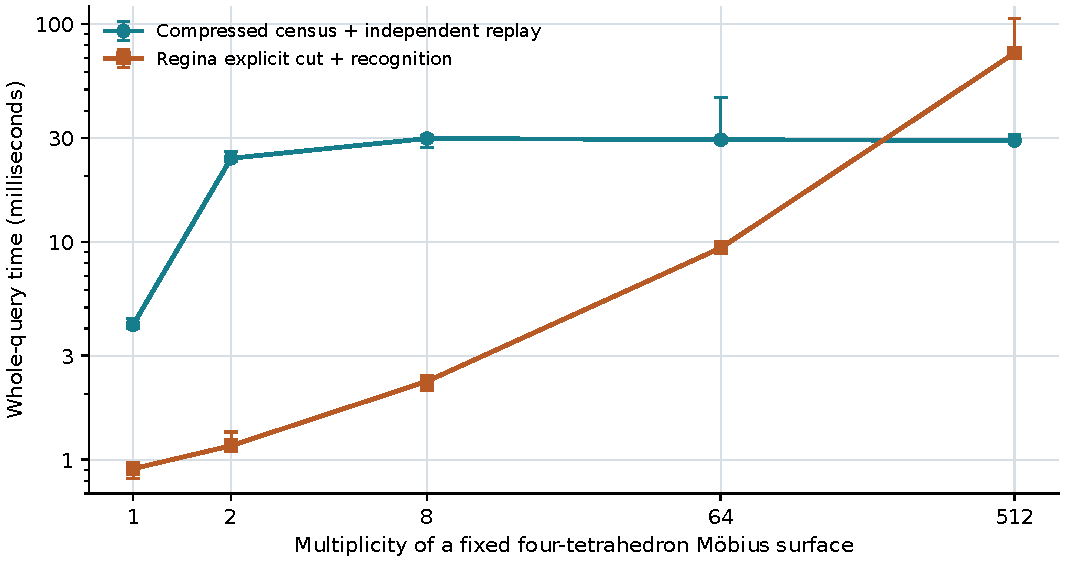
\includegraphics[width=0.94\linewidth]{figures/mobius_capacity.pdf}
\caption{Whole-cut production and verification versus explicit cut and
recognition, on one fixed source with increasing M\"obius multiplicity.
Points are seven-round medians; bars show the observed minimum and maximum.
Both axes are logarithmic. Connecting lines only guide the eye.}
\label{fig:capacity-times}
\end{figure}

On a source with three-handles, the disabled path returns early and does
not do comparable successful work. Its shorter runtime is an abstention
cost and is not used to claim a speedup or slowdown. On the three controls
without three-handles, all three strategies take the identical native
path. Their measured differences are timing variation, not forest work.
The final patch changes the default keyword from BFS to maximum weight
after these measurements; every measured call supplied an explicit
strategy, so that default change does not change the measured operation.

\subsection{Binary capacity and certificate size}

The separate capacity run multiplies the four-tetrahedron M\"obius vector
by $2^{16384}$. Both native strategies certify and independently replay
the exact census
\[
 \left(2^{16383}+1\right)H_1.
\]
The recorded single-run production-plus-replay totals are 0.1003 seconds
for BFS and 0.1088 seconds for maximum weight. Each serialized full
certificate is 5,429,503 bytes. No explicit cut of this input was attempted,
and there is no paired speedup comparison for it.

The full certificate includes the original source and orbit certificates,
which repeat some large integers. Its megabyte size must not be confused
with the added top-forest trace, whose combinatorial size is independent
of the multiplier. The test establishes that this family is handled
without one record per normal disc or component. It does not establish
optimal certificate encoding or the same time for every input of comparable
coordinate bit length. The multiplier itself has 16,385 bits.
An additional integration test cuts the five-tetrahedron loop source by
$2^{16384}$ boundary-link discs and replays the exact census
$2^{16384}H_0\sqcup H_1$.

\subsection{Regression, hostile replay, and exact algebra}

The full integrated native regression suite passes: 1,696 tests in
377.446 seconds, with no failures or errors. This includes the 12 new
dual-forest test methods and six new integration methods. The run used
the pinned repository's historical fixtures and dependent research
directories, not an incomplete extraction of the runtime folder. Its
complete log is included in \code{research/data/native\_regression.log}.


The focused native tests cover repeated interior vertices, both occurrences
of a loop, positive-weight loop splitting, reversed dependent orders,
alternative valid trees, tetrahedron and local-vertex relabelling,
source tampering, forbidden Boolean identifiers, the integer codec,
operation allowances, callback propagation, and scalar-certificate reuse.
The weighted graph producer is checked against every spanning tree on
128 small multigraph instances. Integration tests disable the relevant
producer entry points during complete v6 replay and reject wrapper removal,
nested wrappers, altered source geometry, and mismatched coordinates.

The quotient component has 27 passing tests. These include 400 deterministic
random algebraic instances, 250 independent SymPy rank comparisons, all
32 combinations of zero/nonzero chain dimensions, rational support with
a nonunit denominator, an outside witness with nonunit evaluation,
commuting-square failures, malformed matrices, stale input binding,
hostile witness mutations, and command-line round trips. The additional
16,384-bit subprocess test checks the documented large-decimal launch
configuration. These are checks of the exact algebraic contract, not
geometric examples of the future hierarchy interface.
